\chapter{Requerimientos}
\section{Introducción}
Dentro del aplicativo, se plantean un serie de requerimientos de tipo cliente y tipo desarrollador, que serán abordados y explicados a lo largo de este capítulo.
\section{Requerimientos tipo C}
Los requerimientos tipo C que plantean para el aplicativo son los mostrados en la siguiente imagen:
\begin{figure}[h!]
	\centering
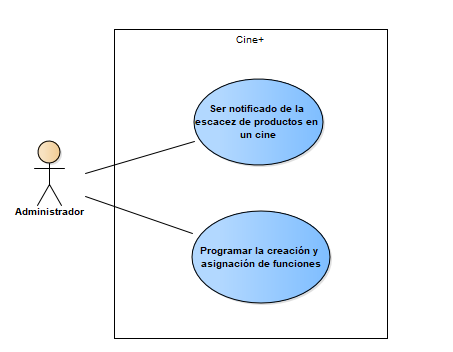
\includegraphics[width=.6\linewidth]{diseno/requerimientos/imgs/casosUso1}
	\caption{Casos de uso del sistema}
\end{figure}
\newpage
\begin{figure}[h!]
	\centering
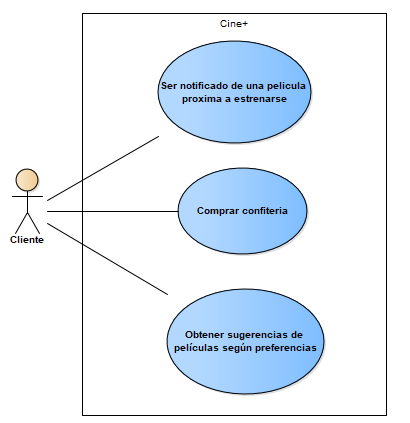
\includegraphics[width=.6\linewidth]{diseno/requerimientos/imgs/casosUso2}
	\caption{Casos de uso del sistema}
\end{figure}

A continuación se espeficarán y describirán cada uno de los casos de uso expuestos:
\begin{figure}[h!]
\centering
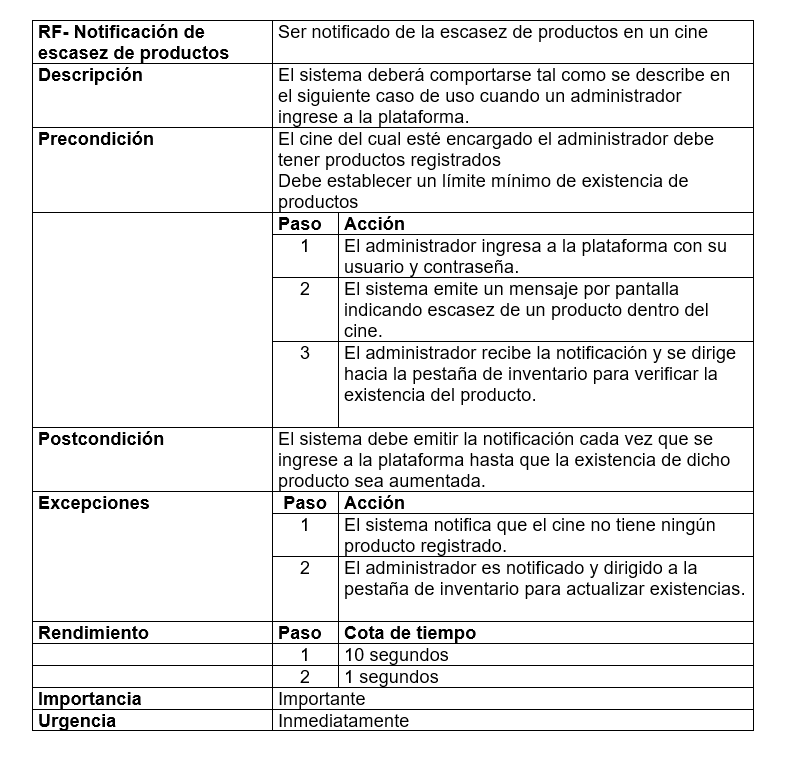
\includegraphics[width=.8\linewidth]{diseno/requerimientos/imgs/casos1}
	%\caption{Especificación casos de uso del sistema}
\end{figure}

\begin{figure}[h!]
	\centering
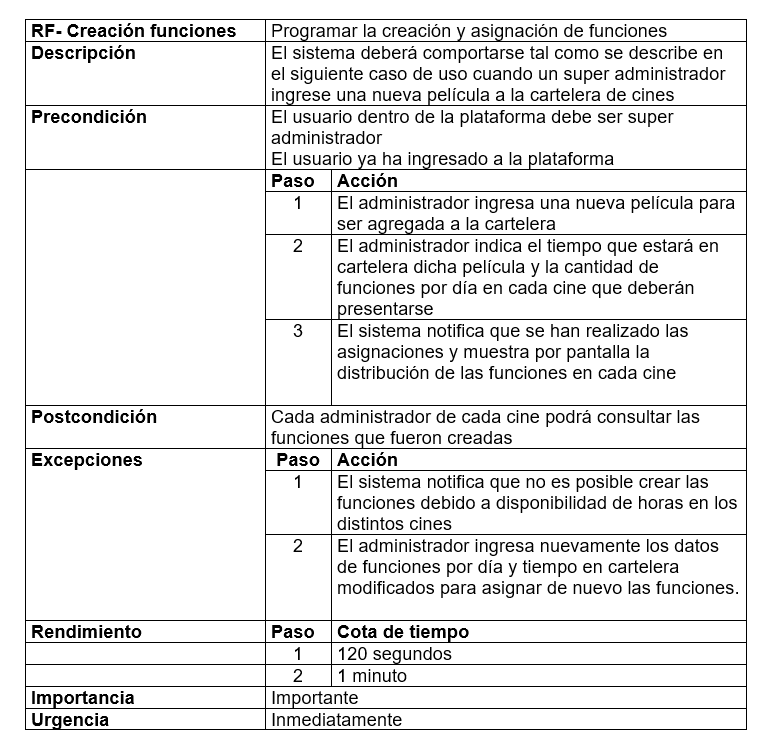
\includegraphics[width=.8\linewidth]{diseno/requerimientos/imgs/casos2}
	%\caption{Especificación casos de uso del sistema}
\end{figure}